
\medskip

\textbf{Partie A}

\medskip

\begin{minipage}{0.75\linewidth}
Tom a acheté un dé équilibré à 12 faces numérotées de 1 à 12.

Il lance ce dé et s'intéresse au résultat qui apparaît sur la face du dessus.

Sur la photo ci-contre de ce dé, le résultat obtenu est 3.
\end{minipage}\hfill
\begin{minipage}{0.21\linewidth}
%\includegraphics[width=2cm]{de12}
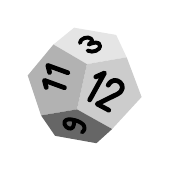
\begin{tikzpicture}[line cap=round,line join=round,scale=0.1]
	\coordinate (1) at (10.075,11.133);
	\coordinate (2) at (5.822,13.625);
	\coordinate (3) at (8.447, 15.762);
	\coordinate (4) at (13.785, 14.843);
	\coordinate (5) at (15.125, 11.997);
	\coordinate (6) at (17.019, 6.958);
	\coordinate (7) at (13.275, 2.893);
	\coordinate (8) at (8.812, 5.385);
	\coordinate (9) at (2.55, 9.688);
	\coordinate (10) at (4.249, 4.614);
	\coordinate (11) at (6.027, 2.029);
	\coordinate (12) at (11.282, 1.09);
	\fill[gray!20]%face 3
	(1) -- (2) -- (3) -- (4) -- (5) -- cycle;
	\path[draw=black,line width=0.5mm]
	(9.178, 13.819).. controls (9.213, 14.428) and (10.238, 14.714) ..
	(10.6, 14.359).. controls (10.926, 14.038) and (10.529, 13.831) ..
	(10.308, 13.629).. controls (10.712, 13.801) and (11.738, 14.181) ..
	(11.748, 13.4).. controls (11.754, 12.984) and (10.864, 12.481) ..
		(10.159, 12.855);

	\fill[gray!40]%face 12
	(1) -- (5) -- (6) -- (7) -- (8) -- cycle;
	\draw[line width=0.6mm] %1 du 12
	(11.21, 9.516) -- (12.306, 10.007) -- (10.425, 6.59);
	\draw[line width=0.6mm] %2 du 12
	(12.776, 8.458).. controls (13.603, 10.034) and (15.596, 8.204) ..
	(13.939, 7.326) -- (11.384, 6.069) -- (12.847, 5.288);

	\fill[gray!60] %face 11
	(1) -- (2) -- (9) -- (10) -- (8) -- cycle;
	\draw[line width=0.6mm] %1
	(4.908, 8.172) -- (4.682, 9.064) -- (7.223, 8.138);
	\draw[line width=0.6mm] %1
	(5.331, 10.075) -- (5.105, 10.967) -- (7.647, 10.041);

	\fill[darkgray!80] %face 9
	(7)-- (8) -- (10) --(11) -- (12) -- cycle;
	\draw[line width=0.5mm]
	(8.464, 3.962).. controls (8.464, 3.962) and (8.501, 3.027) ..
	(8.06, 2.947).. controls (7.639, 2.871) and (7.081, 3.362) ..
	(7.233, 3.813).. controls (7.466, 4.51) and (9.499, 3.89) ..
	(9.725, 3.265).. controls (9.921,	2.723) and (9.457, 2.508) ..
	(9.438, 2.479);
\end{tikzpicture}
\end{minipage}

%\medskip

\begin{enumerate}
\item Expliquer pourquoi la probabilité d'obtenir le nombre 4 est égale à $\dfrac{1}{12}$.
\item Quelle est la probabilité que le résultat obtenu soit un nombre pair ?
\item Tom pense que la probabilité d'obtenir un multiple de 3 est supérieure à 0,3. A-t-il raison ?
\end{enumerate}

\bigskip

\textbf{Partie B}

\medskip

Tom souhaite maintenant simuler le lancer de deux dés équilibrés à 12 faces numérotées de 1 à 12.

Le bloc \og lancer \fg{} simule le lancer des deux dés et calcule la somme obtenue.

Par exemple, si le résultat du dé \no 1 est égal à 3 et que le résultat du dé \no 2 est égal à 5 alors la somme sera égale à 8.

Voici le programme de Tom.

\begin{center}
\begin{tabular}{|>{\centering\arraybackslash}p{5.5cm}|>{\centering\arraybackslash}p{8cm}|}
\hline
&\\
\textbf{Programme} & \textbf{Bloc \og Lancer} \fg\\
&\\
\begin{scratch}[scale=0.85]
\blockinit{Quand \greenflag est cliqué}
\blockmoreblocks{Lancer}
\blockifelse{si\ovaloperator{\ovalvariable{Résultat} >\ovalvariable{6}}  alors}
{\blocklook{dire \ovalnum{Gagné !} pendant \ovalnum{2} secondes}}
{\blocklook{dire \ovalnum{Perdu !} pendant \ovalnum{2} secondes}}
\end{scratch}
&
\begin{scratch}[scale=0.85,num blocks]
\initmoreblocks{définir \namemoreblocks{Lancer}}
\blockvariable{mettre \selectmenu{Dé 1} à \ovaloperator{nombre aléatoire entre \ovalnum{1} et \ovalnum{...}}}
\blockvariable{mettre \selectmenu{Dé 2} à \ovaloperator{nombre aléatoire entre \ovalnum{...} et \ovalnum{12}}}
\blockvariable{mettre \selectmenu{Résultat} à \ovaloperator{\ovalnum{...} + \ovalnum{...}}} 
\end{scratch}
\newline

\emph{On rappelle que l'instruction}
\newline

\ovaloperator{nombre aléatoire entre \ovalnum{1} et \ovalnum{4}} \newline

%\begin{scratch}\blockvariable{\selectmenu{} \ovaloperator{nombre aléatoire entre \ovalnum{1} et \ovalnum{4}}}\end{scratch} \newline

\emph{renvoie au hasard un nombre}\newline
\emph{ parmi $1, 2, 3$ ou $4$.}\\ 
 &\\
 \hline
\end{tabular}

\end{center}
\begin{enumerate}
\item \textbf{Recopier les lignes 2, 3 et 4} du bloc \og Lancer \fg en les complétant.
\item Si le résultat du dé \no 1 est égal à 8 et le résultat du dé \no 2 est égal à 3, qu'affichera le programme ?

Justifier.
\end{enumerate}

